% ==============================================================================
% BỘ ĐỀ THAM KHẢO TUYỂN SINH 10 NĂM HỌC 2026-2027 SỞ GD&ĐT TP.HCM
% ĐỢT 20: CỤM 13 (ĐỀ 3 - ĐỀ SỐ 39) VÀ CỤM 14 (ĐỀ 1 - ĐỀ SỐ 40)
% Gồm 14 bài toán tự luận chuẩn cấu trúc tuyển sinh 10
% ==============================================================================

% ==============================================================================
% CỤM 13 - ĐỀ THAM KHẢO 3 (ĐỀ SỐ 39)
% ==============================================================================

\begin{bt}%[9D6H18-2]
% nguon: Đề tham khảo Tuyển sinh 10 năm học 2026-2027 Sở GD&ĐT TP.HCM - Cụm 13 Đề 3 (Đề số 39)
Cho hàm số $y = \dfrac{1}{4}x^2$ có đồ thị là parabol $(P)$.
\begin{enumerate}[a)]
	\item Vẽ đồ thị $(P)$ trên mặt phẳng toạ độ $Oxy$.
	\item Tìm toạ độ các điểm $M$ thuộc $(P)$ có tung độ gấp $2$ lần hoành độ.
\end{enumerate}
\loigiai{
\begin{enumerate}[a)]
	\item Bảng giá trị tương ứng của $x$ và $y$:
	\begin{center}
		\begin{tabular}{|c|c|c|c|c|c|}
			\hline
			$x$ & $-4$ & $-2$ & $0$ & $2$ & $4$ \\ \hline
			$y = \dfrac{1}{4}x^2$ & $4$ & $1$ & $0$ & $1$ & $4$ \\ \hline
		\end{tabular}
	\end{center}
	Đồ thị $(P)$ là một đường parabol đi qua các điểm $(-4; 4)$, $(-2; 1)$, $(0; 0)$, $(2; 1)$, $(4; 4)$, có đỉnh tại gốc toạ độ $O(0;0)$, nhận trục $Oy$ làm trục đối xứng và quay bề lõm lên trên.
	\begin{center}
	\begin{tikzpicture}[>=stealth,scale=0.8]
		\draw[->] (-5,0) -- (5,0) node[below] {$x$};
		\draw[->] (0,-1) -- (0,5.5) node[left] {$y$};
		\node[below left] at (0,0) {$O$};
		\draw[dashed] (-4,0) node[below] {$-4$} -- (-4,4) -- (0,4) node[left] {$4$} -- (4,4) -- (4,0) node[below] {$4$};
		\draw[dashed] (-2,0) node[below] {$-2$} -- (-2,1) -- (0,1) node[left] {$1$} -- (2,1) -- (2,0) node[below] {$2$};
		\draw[thick,smooth,samples=100,domain=-4.4:4.4] plot(\x,{0.25*(\x)^2});
		\fill (-4,4) circle (1.5pt) (-2,1) circle (1.5pt) (0,0) circle (1.5pt) (2,1) circle (1.5pt) (4,4) circle (1.5pt);
		\node[right] at (3,2.5) {$(P)\colon y = \dfrac{1}{4}x^2$};
	\end{tikzpicture}
	\end{center}
	\item Vì điểm $M$ có tung độ gấp $2$ lần hoành độ nên ta có:
	$$y = 2x.$$
	Thay vào phương trình của $(P)$, ta có:
	$$\dfrac{1}{4}x^2 = 2x \iff \dfrac{1}{4}x^2 - 2x = 0 \iff x\left(\dfrac{1}{4}x - 2\right) = 0 \iff x = 0 \text{ hoặc } x = 8.$$
	\begin{itemize}
		\item Với $x = 0 \implies y = 0$.
		\item Với $x = 8 \implies y = 2 \cdot 8 = 16$.
	\end{itemize}
	Vậy toạ độ các điểm cần tìm là $(0; 0)$ và $(8; 16)$.
\end{enumerate}
}
\end{bt}

\begin{bt}%[9D6H20-2]
% nguon: Đề tham khảo Tuyển sinh 10 năm học 2026-2027 Sở GD&ĐT TP.HCM - Cụm 13 Đề 3 (Đề số 39)
Cho phương trình $x^2 + 9x - 8 = 0$.
\begin{enumerate}[a)]
	\item Chứng minh rằng phương trình luôn có hai nghiệm phân biệt $x_1, x_2$.
	\item Không giải phương trình, hãy tính giá trị của biểu thức $A = \dfrac{x_1}{x_2} + \dfrac{x_2}{x_1}$.
\end{enumerate}
\loigiai{
\begin{enumerate}[a)]
	\item Phương trình $x^2 + 9x - 8 = 0$ có các hệ số $a = 1$, $b = 9$, $c = -8$.
	Biệt thức $\Delta$ của phương trình:
	$$\Delta = b^2 - 4ac = 9^2 - 4 \cdot 1 \cdot (-8) = 81 + 32 = 113 > 0.$$
	(hoặc do $a \cdot c = 1 \cdot (-8) = -8 < 0$ nên phương trình có hai nghiệm trái dấu).
	Vì $\Delta > 0$ nên phương trình luôn có hai nghiệm phân biệt $x_1, x_2$.
	\item Áp dụng định lý Viète, ta có:
	$$\begin{cases} x_1 + x_2 = -\dfrac{b}{a} = -9 \\ x_1 x_2 = \dfrac{c}{a} = -8. \end{cases}$$
	Ta có:
	$$x_1^2 + x_2^2 = (x_1 + x_2)^2 - 2x_1 x_2 = (-9)^2 - 2(-8) = 81 + 16 = 97.$$
	Khi đó:
	$$A = \dfrac{x_1}{x_2} + \dfrac{x_2}{x_1} = \dfrac{x_1^2 + x_2^2}{x_1 x_2} = \dfrac{97}{-8} = -\dfrac{97}{8}.$$
	Vậy $A = -\dfrac{97}{8}$.
\end{enumerate}
}
\end{bt}

\begin{bt}%[9D8H26-3]
% nguon: Đề tham khảo Tuyển sinh 10 năm học 2026-2027 Sở GD&ĐT TP.HCM - Cụm 13 Đề 3 (Đề số 39)
Bạn An ghi lại điểm kiểm tra giữa kì I môn Toán của $30$ bạn học sinh trong lớp như sau:
\begin{center}
\begin{tabular}{cccccccccc}
	$6$ & $7$ & $9$ & $9$ & $10$ & $8$ & $8$ & $6$ & $9$ & $7$ \\
	$8$ & $9$ & $7$ & $6$ & $10$ & $7$ & $7$ & $8$ & $9$ & $7$ \\
	$10$ & $8$ & $9$ & $7$ & $9$ & $9$ & $8$ & $7$ & $8$ & $9$
\end{tabular}
\end{center}
\begin{enumerate}[a)]
	\item Lập bảng tần số cho mẫu số liệu trên.
	\item Tính điểm trung bình của các bạn học sinh trong bảng.
	\item Chọn ngẫu nhiên một bạn học sinh trong danh sách. Tính xác suất để bạn đó có điểm kiểm tra môn Toán từ $9$ điểm trở lên.
\end{enumerate}
\loigiai{
\begin{enumerate}[a)]
	\item Bảng tần số của mẫu số liệu:
	\begin{center}
		\begin{tabular}{|l|c|c|c|c|c|c|}
			\hline
			Điểm số ($x$) & $6$ & $7$ & $8$ & $9$ & $10$ & Cộng \\ \hline
			Tần số ($n$) & $3$ & $8$ & $7$ & $9$ & $3$ & $N = 30$ \\ \hline
		\end{tabular}
	\end{center}
	\item Điểm trung bình của các bạn học sinh là:
	$$\bar{x} = \dfrac{6 \cdot 3 + 7 \cdot 8 + 8 \cdot 7 + 9 \cdot 9 + 10 \cdot 3}{30} = \dfrac{18 + 56 + 56 + 81 + 30}{30} = \dfrac{241}{30} \approx 8{,}03.$$
	\item Không gian mẫu có số phần tử là $n(\Omega) = 30$.
	Gọi $A$ là biến cố: ``Bạn học sinh được chọn có điểm kiểm tra từ $9$ điểm trở lên''.
	Các bạn đạt từ $9$ điểm trở lên gồm những bạn đạt điểm $9$ và điểm $10$.
	Số học sinh đạt điểm $9$ hoặc $10$ là:
	$$n(A) = 9 + 3 = 12.$$
	Xác suất của biến cố $A$ là:
	$$P(A) = \dfrac{n(A)}{n(\Omega)} = \dfrac{12}{30} = \dfrac{2}{5}.$$
\end{enumerate}
}
\end{bt}

\begin{bt}%[9D6V21-3]
% nguon: Đề tham khảo Tuyển sinh 10 năm học 2026-2027 Sở GD&ĐT TP.HCM - Cụm 13 Đề 3 (Đề số 39)
Một trường học xây dựng sân bóng rổ hình chữ nhật có kích thước $14\text{ m} \times 26\text{ m}$. Theo thiết kế, người ta cũng xây dựng một lối đi có chiều rộng là $x$ (m) chạy dọc theo hai cạnh liên tiếp của sân bóng rổ.
\begin{enumerate}[a)]
	\item Viết biểu thức $S$ biểu diễn diện tích của lối đi theo $x$.
	\item Bạn An đi bộ từ cửa vào đến cửa ra và đi dọc theo mép ngoài của lối đi. Hãy tính quãng đường An đã đi, biết diện tích của lối đi theo thiết kế là $129\text{ m}^2$.
\end{enumerate}
\loigiai{
\begin{enumerate}[a)]
	\item Lối đi bao gồm một phần hình chữ nhật dọc kích thước $14\text{ m} \times x\text{ m}$ và một phần hình chữ nhật ngang tính cả góc vuông có kích thước $(26 + x)\text{ m} \times x\text{ m}$.
	Do đó biểu thức tính diện tích lối đi theo $x$ là:
	$$S = 14x + x(26 + x) = 14x + 26x + x^2 = x^2 + 40x\text{ (m}^2\text{)}.$$
	\item Vì diện tích của lối đi là $129\text{ m}^2$ nên ta có phương trình:
	$$x^2 + 40x = 129 \iff x^2 + 40x - 129 = 0.$$
	Phương trình có $\Delta' = 20^2 - 1 \cdot (-129) = 400 + 129 = 529 > 0 \implies \sqrt{\Delta'} = 23$.
	Do đó phương trình có hai nghiệm:
	$$x_1 = -20 + 23 = 3\text{ (nhận do } x > 0\text{)}; \quad x_2 = -20 - 23 = -43\text{ (loại)}.$$
	Quãng đường An đi bộ dọc theo mép ngoài của lối đi gồm chiều dài cạnh dọc phía ngoài là $14 + x$ (m) và chiều dài cạnh ngang phía ngoài là $26 + x$ (m):
	$$s = (14 + 3) + (26 + 3) = 17 + 29 = 46\text{ (m)}.$$
	Vậy quãng đường bạn An đã đi là $46$ m.
\end{enumerate}
}
\end{bt}

\begin{bt}%[9H0V31-3]
% nguon: Đề tham khảo Tuyển sinh 10 năm học 2026-2027 Sở GD&ĐT TP.HCM - Cụm 13 Đề 3 (Đề số 39)
\begin{enumerate}[a)]
	\item Tính độ dài cung tròn $60^\circ$ của một đường tròn có đường kính $10\text{ cm}$. Biết công thức tính độ dài cung tròn là $l = \dfrac{\pi R n}{180}$, trong đó $R$ là bán kính đường tròn và $n$ là số đo độ của cung.
	\item Một lon nước ngọt hình trụ kiểu dáng mới cao $14\text{ cm}$ và có đường kính đáy là $6\text{ cm}$. Hỏi lon nước ngọt này có thể chứa được hết lượng nước ngọt của một lon cỡ phổ biến trên thế giới thường chứa $335\text{ ml}$ chất lỏng hay không? Vì sao?
\end{enumerate}
\loigiai{
\begin{enumerate}[a)]
	\item Bán kính của đường tròn là:
	$$R = 10 : 2 = 5\text{ (cm)}.$$
	Độ dài cung tròn $60^\circ$ là:
	$$l = \dfrac{\pi \cdot 5 \cdot 60}{180} = \dfrac{5\pi}{3}\text{ (cm)} \approx 5{,}24\text{ (cm)}.$$
	\item Lon nước ngọt hình trụ có bán kính đáy là:
	$$r = 6 : 2 = 3\text{ (cm)}.$$
	Thể tích của lon nước ngọt này là:
	$$V = \pi r^2 h = \pi \cdot 3^2 \cdot 14 = 126\pi\text{ (cm}^3\text{)}.$$
	Vì $1\text{ cm}^3 = 1\text{ ml}$ nên:
	$$V = 126\pi\text{ (ml)} \approx 126 \cdot 3{,}1416 \approx 395{,}84\text{ (ml)}.$$
	Vì $395{,}84\text{ ml} > 335\text{ ml}$ nên lon nước ngọt dáng cao này hoàn toàn có thể chứa hết lượng nước ngọt của lon cỡ phổ biến $335\text{ ml}$.
\end{enumerate}
}
\end{bt}

\begin{bt}%[9D1H3-4]
% nguon: Đề tham khảo Tuyển sinh 10 năm học 2026-2027 Sở GD&ĐT TP.HCM - Cụm 13 Đề 3 (Đề số 39)
Một khu đất hình chữ nhật có chu vi bằng $120$ m. Trong đợt giải toả đất làm đường cao tốc, chiều dài khu đất bị lấy vào $7$ m để làm đường, do đó chiều dài còn lại bằng $4{,}3$ lần chiều rộng. Tính diện tích của khu đất lúc ban đầu.
\loigiai{
Nửa chu vi của khu đất hình chữ nhật là:
$$120 : 2 = 60\text{ (m)}.$$
Gọi $x$ (m) là chiều dài lúc đầu và $y$ (m) là chiều rộng lúc đầu của khu đất ($x > 7, y > 0$).
Vì tổng chiều dài và chiều rộng bằng nửa chu vi nên ta có phương trình:
$$x + y = 60. \quad (1)$$
Chiều dài còn lại của khu đất sau khi bị cắt bớt $7$ m là:
$$x - 7\text{ (m)}.$$
Vì chiều dài còn lại bằng $4{,}3$ lần chiều rộng nên ta có phương trình:
$$x - 7 = 4{,}3y \iff x - 4{,}3y = 7. \quad (2)$$
Từ $(1)$ và $(2)$ ta có hệ phương trình:
$$\begin{cases} x + y = 60 \\ x - 4{,}3y = 7 \end{cases} \iff \begin{cases} 5{,}3y = 53 \\ x + y = 60 \end{cases} \iff \begin{cases} y = 10 \\ x = 50 \end{cases}\text{ (thoả mãn)}.$$
Vậy lúc đầu khu đất có chiều dài là $50$ m và chiều rộng là $10$ m.
Diện tích khu đất ban đầu là:
$$S = 50 \cdot 10 = 500\text{ (m}^2\text{)}.$$
}
\end{bt}

\begin{bt}%[9H9C29-3]
% nguon: Đề tham khảo Tuyển sinh 10 năm học 2026-2027 Sở GD&ĐT TP.HCM - Cụm 13 Đề 3 (Đề số 39)
Cho tam giác $ABC$ nhọn ($AB < AC$) nội tiếp đường tròn $(O; R)$, có đường cao $AH$. Gọi $M, N$ lần lượt là hình chiếu của điểm $H$ trên cạnh $AB$ và $AC$.
\begin{enumerate}[a)]
	\item Chứng minh rằng tứ giác $AMHN$ là tứ giác nội tiếp.
	\item Chứng minh rằng $AM \cdot AB = AH^2$. Từ đó suy ra $AM \cdot AB = AN \cdot AC$.
	\item Cho biết $\widehat{BAC} = 60^\circ$ và $R = 3\text{ cm}$. Tính diện tích hình quạt tròn tạo bởi hai bán kính $OB, OC$ ứng với cung nhỏ $BC$.
\end{enumerate}
\loigiai{
\begin{center}
\begin{tikzpicture}[>=stealth,scale=1.1]
	\def\R{2.4}
	\coordinate (O) at (0,0);
	\draw[thick] (O) circle (\R);
	\coordinate (A) at (0.4,2.36);
	\coordinate (B) at (-2.1,-1.16);
	\coordinate (C) at (1.8,-1.58);
	\draw (A) -- (B) -- (C) -- cycle;
	% Đường cao AH
	\coordinate (H) at ($(B)!(A)!(C)$);
	\draw (A) -- (H);
	% Hình chiếu M, N
	\coordinate (M) at ($(A)!(H)!(B)$);
	\coordinate (N) at ($(A)!(H)!(C)$);
	\draw (H) -- (M);
	\draw (H) -- (N);
	\draw (M) -- (N);
	\draw (O) -- (B);
	\draw (O) -- (C);
	% Ký hiệu
	\fill (O) circle (1.5pt) node[below] {$O$}
		  (A) circle (1.5pt) node[above] {$A$}
		  (B) circle (1.5pt) node[left] {$B$}
		  (C) circle (1.5pt) node[right] {$C$}
		  (H) circle (1.5pt) node[below] {$H$}
		  (M) circle (1.5pt) node[above left] {$M$}
		  (N) circle (1.5pt) node[above right] {$N$};
\end{tikzpicture}
\end{center}
\begin{enumerate}[a)]
	\item Vì $M$ là hình chiếu của $H$ trên $AB$ nên $HM \perp AB \implies \widehat{AMH} = 90^\circ$.
	Tam giác $AMH$ vuông tại $M$ nên nội tiếp đường tròn đường kính $AH$.
	Vì $N$ là hình chiếu của $H$ trên $AC$ nên $HN \perp AC \implies \widehat{ANH} = 90^\circ$.
	Tam giác $ANH$ vuông tại $N$ nên nội tiếp đường tròn đường kính $AH$.
	Suy ra bốn điểm $A, M, H, N$ cùng thuộc đường tròn đường kính $AH$, hay tứ giác $AMHN$ nội tiếp.
	\item Xét $\triangle AHM$ và $\triangle ABH$ có:
	\begin{itemize}
		\item $\widehat{BAH}$ là góc chung;
		\item $\widehat{AMH} = \widehat{AHB} = 90^\circ$.
	\end{itemize}
	Do đó $\triangle AHM \sim \triangle ABH$ (g-g).
	Suy ra $\dfrac{AH}{AB} = \dfrac{AM}{AH} \implies AM \cdot AB = AH^2$.
	Chứng minh tương tự, xét $\triangle AHN$ và $\triangle ACH$ có:
	\begin{itemize}
		\item $\widehat{CAH}$ là góc chung;
		\item $\widehat{ANH} = \widehat{AHC} = 90^\circ$.
	\end{itemize}
	Do đó $\triangle AHN \sim \triangle ACH$ (g-g).
	Suy ra $\dfrac{AH}{AC} = \dfrac{AN}{AH} \implies AN \cdot AC = AH^2$.
	Từ đó suy ra $AM \cdot AB = AN \cdot AC = AH^2$.
	\item Trong đường tròn $(O)$, góc nội tiếp $\widehat{BAC}$ và góc ở tâm $\widehat{BOC}$ cùng chắn cung nhỏ $BC$, do đó:
	$$\widehat{BOC} = 2\widehat{BAC} = 2 \cdot 60^\circ = 120^\circ.$$
	Diện tích hình quạt tròn ứng với cung nhỏ $BC$ là:
	$$S_q = \dfrac{\pi R^2 n}{360} = \dfrac{\pi \cdot 3^2 \cdot 120}{360} = \dfrac{9\pi}{3} = 3\pi\text{ (cm}^2\text{)} \approx 9{,}42\text{ (cm}^2\text{)}.$$
	Vậy diện tích hình quạt tròn cần tìm là $3\pi\text{ cm}^2$.
\end{enumerate}
}
\end{bt}

% ==============================================================================
% CỤM 14 - ĐỀ THAM KHẢO 1 (ĐỀ SỐ 40)
% ==============================================================================

\begin{bt}%[9D6H18-2]
% nguon: Đề tham khảo Tuyển sinh 10 năm học 2026-2027 Sở GD&ĐT TP.HCM - Cụm 14 Đề 1 (Đề số 40)
Cho hàm số $y = \dfrac{1}{4}x^2$ có đồ thị là parabol $(P)$.
\begin{enumerate}[a)]
	\item Vẽ đồ thị $(P)$ trên mặt phẳng toạ độ $Oxy$.
	\item Tìm toạ độ các điểm $M$ thuộc đồ thị $(P)$ có tung độ bằng $2$ lần hoành độ.
\end{enumerate}
\loigiai{
\begin{enumerate}[a)]
	\item Bảng giá trị của hàm số:
	\begin{center}
		\begin{tabular}{|c|c|c|c|c|c|}
			\hline
			$x$ & $-4$ & $-2$ & $0$ & $2$ & $4$ \\ \hline
			$y = \dfrac{1}{4}x^2$ & $4$ & $1$ & $0$ & $1$ & $4$ \\ \hline
		\end{tabular}
	\end{center}
	Đồ thị $(P)$ là đường parabol có đỉnh tại gốc toạ độ $O(0;0)$, nhận trục $Oy$ làm trục đối xứng và đi qua các điểm $(-4; 4)$, $(-2; 1)$, $(0; 0)$, $(2; 1)$, $(4; 4)$.
	\begin{center}
	\begin{tikzpicture}[>=stealth,scale=0.8]
		\draw[->] (-5,0) -- (5,0) node[below] {$x$};
		\draw[->] (0,-1) -- (0,5.5) node[left] {$y$};
		\node[below left] at (0,0) {$O$};
		\draw[dashed] (-4,0) node[below] {$-4$} -- (-4,4) -- (0,4) node[left] {$4$} -- (4,4) -- (4,0) node[below] {$4$};
		\draw[dashed] (-2,0) node[below] {$-2$} -- (-2,1) -- (0,1) node[left] {$1$} -- (2,1) -- (2,0) node[below] {$2$};
		\draw[thick,smooth,samples=100,domain=-4.4:4.4] plot(\x,{0.25*(\x)^2});
		\fill (-4,4) circle (1.5pt) (-2,1) circle (1.5pt) (0,0) circle (1.5pt) (2,1) circle (1.5pt) (4,4) circle (1.5pt);
		\node[right] at (3,2.5) {$(P)\colon y = \dfrac{1}{4}x^2$};
	\end{tikzpicture}
	\end{center}
	\item Điểm $M$ thuộc $(P)$ có tung độ bằng $2$ lần hoành độ nên ta có $y = 2x$.
	Phương trình hoành độ giao điểm:
	$$2x = \dfrac{1}{4}x^2 \iff \dfrac{1}{4}x^2 - 2x = 0 \iff x(x - 8) = 0 \iff x = 0 \text{ hoặc } x = 8.$$
	\begin{itemize}
		\item Với $x = 0 \implies y = 0$.
		\item Với $x = 8 \implies y = 2 \cdot 8 = 16$.
	\end{itemize}
	Vậy toạ độ các điểm cần tìm là $(0; 0)$ và $(8; 16)$.
\end{enumerate}
}
\end{bt}

\begin{bt}%[9D6H20-2]
% nguon: Đề tham khảo Tuyển sinh 10 năm học 2026-2027 Sở GD&ĐT TP.HCM - Cụm 14 Đề 1 (Đề số 40)
Cho phương trình $x^2 - 4x + 3 = 0$.
\begin{enumerate}[a)]
	\item Chứng minh phương trình luôn có hai nghiệm phân biệt $x_1, x_2$.
	\item Không giải phương trình, hãy tính giá trị của biểu thức $A = \dfrac{5x_1 - x_2}{x_1} - \dfrac{x_1 - 5x_2}{x_2}$.
\end{enumerate}
\loigiai{
\begin{enumerate}[a)]
	\item Phương trình $x^2 - 4x + 3 = 0$ có các hệ số $a = 1$, $b = -4$, $c = 3$.
	Ta có:
	$$\Delta' = (-2)^2 - 1 \cdot 3 = 4 - 3 = 1 > 0.$$
	Vì $\Delta' > 0$ nên phương trình luôn có hai nghiệm phân biệt $x_1, x_2$.
	\item Theo định lý Viète, ta có:
	$$\begin{cases} x_1 + x_2 = -\dfrac{b}{a} = 4 \\ x_1 x_2 = \dfrac{c}{a} = 3. \end{cases}$$
	Ta có:
	$$x_1^2 + x_2^2 = (x_1 + x_2)^2 - 2x_1 x_2 = 4^2 - 2 \cdot 3 = 16 - 6 = 10.$$
	Biến đổi biểu thức $A$:
	\begin{align*}
		A &= \dfrac{5x_1 - x_2}{x_1} - \dfrac{x_1 - 5x_2}{x_2} \\
		&= \dfrac{x_2(5x_1 - x_2) - x_1(x_1 - 5x_2)}{x_1 x_2} \\
		&= \dfrac{5x_1 x_2 - x_2^2 - x_1^2 + 5x_1 x_2}{x_1 x_2} \\
		&= \dfrac{10x_1 x_2 - (x_1^2 + x_2^2)}{x_1 x_2}.
	\end{align*}
	Thay số vào, ta được:
	$$A = \dfrac{10 \cdot 3 - 10}{3} = \dfrac{20}{3}.$$
	Vậy $A = \dfrac{20}{3}$.
\end{enumerate}
}
\end{bt}

\begin{bt}%[9D8H26-3]
% nguon: Đề tham khảo Tuyển sinh 10 năm học 2026-2027 Sở GD&ĐT TP.HCM - Cụm 14 Đề 1 (Đề số 40)
Một bó hoa gồm $5$ bông hoa màu đỏ và $3$ bông hoa màu vàng. Bạn Linh chọn ngẫu nhiên cùng lúc $4$ bông hoa từ bó hoa đó.
\begin{enumerate}[a)]
	\item Liệt kê các cách chọn (theo số lượng hoa mỗi màu) mà bạn Linh có thể thực hiện.
	\item Tính xác suất của mỗi biến cố sau:
	\begin{itemize}
		\item $A$: ``Trong $4$ bông hoa được chọn ra, có đúng $1$ bông hoa màu đỏ''.
		\item $B$: ``Trong $4$ bông hoa được chọn ra, có ít nhất $1$ bông hoa màu đỏ''.
	\end{itemize}
\end{enumerate}
\loigiai{
\begin{enumerate}[a)]
	\item Các cách chọn $4$ bông hoa từ bó hoa gồm $5$ bông đỏ và $3$ bông vàng là:
	\begin{itemize}
		\item Chọn $4$ bông hoa màu đỏ và $0$ bông hoa màu vàng.
		\item Chọn $3$ bông hoa màu đỏ và $1$ bông hoa màu vàng.
		\item Chọn $2$ bông hoa màu đỏ và $2$ bông hoa màu vàng.
		\item Chọn $1$ bông hoa màu đỏ và $3$ bông hoa màu vàng.
	\end{itemize}
	\item Số cách chọn $4$ bông hoa bất kỳ từ $8$ bông hoa là:
	$$n(\Omega) = \mathrm{C}_8^4 = \dfrac{8 \cdot 7 \cdot 6 \cdot 5}{4 \cdot 3 \cdot 2 \cdot 1} = 70.$$
	\begin{itemize}
		\item Biến cố $A$: ``Có đúng $1$ bông hoa màu đỏ''.
		Số kết quả thuận lợi cho biến cố $A$ là chọn $1$ bông đỏ trong $5$ bông đỏ và $3$ bông vàng trong $3$ bông vàng:
		$$n(A) = \mathrm{C}_5^1 \cdot \mathrm{C}_3^3 = 5 \cdot 1 = 5.$$
		Xác suất của biến cố $A$ là:
		$$P(A) = \dfrac{n(A)}{n(\Omega)} = \dfrac{5}{70} = \dfrac{1}{14}.$$
		\item Biến cố $B$: ``Có ít nhất $1$ bông hoa màu đỏ''.
		Vì cả bó hoa chỉ có $3$ bông màu vàng nên khi chọn ra $4$ bông hoa bất kỳ thì chắc chắn phải có ít nhất $1$ bông hoa màu đỏ.
		Do đó $B$ là biến cố chắc chắn, suy ra:
		$$P(B) = 1.$$
	\end{itemize}
\end{enumerate}
}
\end{bt}

\begin{bt}%[9H0V31-3]
% nguon: Đề tham khảo Tuyển sinh 10 năm học 2026-2027 Sở GD&ĐT TP.HCM - Cụm 14 Đề 1 (Đề số 40)
Quả bóng tennis loại $1$ có đường kính $2{,}5\text{ inch}$ tương ứng với $6{,}35\text{ cm}$ được đựng vừa khít $3$ quả trong một hộp nhựa hình trụ.
Biết diện tích bề mặt hình cầu là $S = 4\pi R^2$ và thể tích hình trụ là $V = \pi r^2 h$.
\begin{enumerate}[a)]
	\item Hãy tính diện tích bề mặt của một quả bóng tennis loại $1$.
	\item Hộp nhựa xếp vừa đủ $3$ quả bóng có thể tích là bao nhiêu?
\end{enumerate}
\loigiai{
\begin{enumerate}[a)]
	\item Bán kính của quả bóng tennis hình cầu là:
	$$R = 6{,}35 : 2 = 3{,}175\text{ (cm)}.$$
	Diện tích bề mặt của một quả bóng tennis là:
	$$S = 4\pi R^2 = 4\pi \cdot (3{,}175)^2 = 40{,}3225\pi\text{ (cm}^2\text{)} \approx 126{,}68\text{ (cm}^2\text{)}.$$
	\item Vì hộp nhựa hình trụ xếp vừa khít $3$ quả bóng tennis nên:
	\begin{itemize}
		\item Bán kính đáy của hình trụ đúng bằng bán kính quả bóng: $r = R = 3{,}175\text{ (cm)}$.
		\item Chiều cao của hình trụ đúng bằng tổng đường kính của $3$ quả bóng:
		$$h = 3 \cdot 6{,}35 = 19{,}05\text{ (cm)}.$$
	\end{itemize}
	Thể tích của hộp nhựa hình trụ là:
	$$V = \pi r^2 h = \pi \cdot (3{,}175)^2 \cdot 19{,}05 = 192{,}03590625\pi\text{ (cm}^3\text{)} \approx 603{,}3\text{ (cm}^3\text{)}.$$
	Vậy hộp nhựa có thể tích là $192{,}03590625\pi\text{ cm}^3$ (xấp xỉ $603{,}3\text{ cm}^3$).
\end{enumerate}
}
\end{bt}

\begin{bt}%[9D6V21-3]
% nguon: Đề tham khảo Tuyển sinh 10 năm học 2026-2027 Sở GD&ĐT TP.HCM - Cụm 14 Đề 1 (Đề số 40)
Một vườn hoa hình vuông có cạnh $10$ m. Người ta làm lối đi trong vườn hoa theo hình chữ thập có chiều rộng là $x$ (m) ($0 < x < 10$).
\begin{enumerate}[a)]
	\item Viết biểu thức biểu thị diện tích còn lại để trồng hoa sau khi làm lối đi.
	\item Biết rằng sau khi làm lối đi thì diện tích còn lại của khu vườn trồng hoa là $81\text{ m}^2$. Tính chiều rộng $x$ của lối đi.
\end{enumerate}
\loigiai{
\begin{enumerate}[a)]
	\item Diện tích của toàn bộ khu vườn hình vuông là:
	$$S_{\text{vườn}} = 10 \cdot 10 = 100\text{ (m}^2\text{)}.$$
	Lối đi hình chữ thập gồm hai dải hình chữ nhật kích thước $10\text{ m} \times x\text{ m}$ giao nhau ở ô vuông chính giữa có diện tích $x^2\text{ (m}^2\text{)}$.
	Diện tích của lối đi là:
	$$S_{\text{lối đi}} = 10x + 10x - x^2 = 20x - x^2\text{ (m}^2\text{)}.$$
	Diện tích còn lại để trồng hoa là:
	$$S = S_{\text{vườn}} - S_{\text{lối đi}} = 100 - (20x - x^2) = x^2 - 20x + 100 = (10 - x)^2\text{ (m}^2\text{)}.$$
	\item Theo đề bài, diện tích trồng hoa còn lại là $81\text{ m}^2$ nên ta có phương trình:
	$$(10 - x)^2 = 81.$$
	Vì $0 < x < 10$ nên $10 - x > 0$, do đó:
	$$10 - x = 9 \iff x = 1\text{ (thoả mãn condition)}.$$
	Vậy chiều rộng của lối đi là $1$ m.
\end{enumerate}
}
\end{bt}

\begin{bt}%[9D1H3-4]
% nguon: Đề tham khảo Tuyển sinh 10 năm học 2026-2027 Sở GD&ĐT TP.HCM - Cụm 14 Đề 1 (Đề số 40)
Thép không gỉ Ferritic là họ thép hợp kim chứa từ $12\%$ đến $27\%$ crôm. Một nhà máy luyện thép hiện có sẵn một lượng hợp kim thép chứa $10\%$ crôm và một lượng hợp kim thép chứa $30\%$ crôm (các nguyên liệu không bị hao hụt trong quá trình luyện).
\begin{enumerate}[a)]
	\item Tính khối lượng hợp kim thép mỗi loại cần dùng để luyện được $500$ tấn thép chứa $16\%$ crôm.
	\item Nhà máy dự định luyện ra loại thép không gỉ Ferritic từ $100$ tấn thép chứa $10\%$ crôm và $x$ tấn thép chứa $30\%$ crôm. Hỏi $x$ phải nằm trong khoảng nào?
\end{enumerate}
\loigiai{
\begin{enumerate}[a)]
	\item Gọi $a$ (tấn) là khối lượng thép chứa $10\%$ crôm và $b$ (tấn) là khối lượng thép chứa $30\%$ crôm cần dùng ($a, b > 0$).
	Vì tổng khối lượng thép cần luyện là $500$ tấn nên ta có phương trình:
	$$a + b = 500. \quad (1)$$
	Khối lượng crôm nguyên chất trong $500$ tấn thép $16\%$ là:
	$$500 \cdot 16\% = 80\text{ (tấn)}.$$
	Tổng lượng crôm từ hai loại thép là:
	$$10\%a + 30\%b = 80 \iff 0{,}1a + 0{,}3b = 80. \quad (2)$$
	Từ $(1)$ và $(2)$ ta có hệ phương trình:
	$$\begin{cases} a + b = 500 \\ 0{,}1a + 0{,}3b = 80 \end{cases} \iff \begin{cases} 0{,}1a + 0{,}1b = 50 \\ 0{,}1a + 0{,}3b = 80 \end{cases} \iff \begin{cases} 0{,}2b = 30 \\ a + b = 500 \end{cases} \iff \begin{cases} b = 150 \\ a = 350 \end{cases}\text{ (thoả mãn)}.$$
	Vậy cần $350$ tấn thép chứa $10\%$ crôm và $150$ tấn thép chứa $30\%$ crôm.
	\item Tổng khối lượng thép thu được là:
	$$100 + x\text{ (tấn)}.$$
	Tổng khối lượng crôm trong hỗn hợp thép là:
	$$100 \cdot 10\% + x \cdot 30\% = 10 + 0{,}3x\text{ (tấn)}.$$
	Tỉ lệ phần trăm crôm trong sản phẩm thép là:
	$$\dfrac{10 + 0{,}3x}{100 + x}.$$
	Để thép thu được thuộc họ thép không gỉ Ferritic (chứa từ $12\%$ đến $27\%$ crôm), ta có bất phương trình kép:
	$$0{,}12 \le \dfrac{10 + 0{,}3x}{100 + x} \le 0{,}27.$$
	Vì $x > 0$ nên $100 + x > 0$:
	\begin{itemize}
		\item Với $0{,}12 \le \dfrac{10 + 0{,}3x}{100 + x} \iff 0{,}12(100 + x) \le 10 + 0{,}3x \iff 12 + 0{,}12x \le 10 + 0{,}3x \iff 0{,}18x \ge 2 \iff x \ge \dfrac{100}{9}$.
		\item Với $\dfrac{10 + 0{,}3x}{100 + x} \le 0{,}27 \iff 10 + 0{,}3x \le 0{,}27(100 + x) \iff 10 + 0{,}3x \le 27 + 0{,}27x \iff 0{,}03x \le 17 \iff x \le \dfrac{1700}{3}$.
	\end{itemize}
	Vậy $x$ nằm trong khoảng $\dfrac{100}{9} \le x \le \dfrac{1700}{3}$ (tấn).
\end{enumerate}
}
\end{bt}

\begin{bt}%[9H9C29-3]
% nguon: Đề tham khảo Tuyển sinh 10 năm học 2026-2027 Sở GD&ĐT TP.HCM - Cụm 14 Đề 1 (Đề số 40)
Từ điểm $S$ nằm ngoài đường tròn $(O; R)$ vẽ hai tiếp tuyến $SM, SN$ đến $(O)$ ($M, N$ là các tiếp điểm). Gọi $H$ là giao điểm của đoạn thẳng $SO$ và dây cung $MN$; $K$ là giao điểm của đoạn thẳng $SO$ và đường tròn $(O)$.
\begin{enumerate}[a)]
	\item Chứng minh tứ giác $SMON$ nội tiếp đường tròn.
	\item Chứng minh $MK$ là tia phân giác của góc $\widehat{SMH}$, từ đó suy ra $MH \cdot KS = KH \cdot MS$.
	\item Biết $OS = R\sqrt{5}$. Tính bán kính đường tròn nội tiếp tam giác $SMN$ theo $R$.
\end{enumerate}
\loigiai{
\begin{center}
\begin{tikzpicture}[>=stealth,scale=1.1]
	\def\R{2.2}
	\coordinate (O) at (0,0);
	\draw[thick] (O) circle (\R);
	% OS = R*sqrt(5) -> S ở (-R*sqrt(5), 0)
	\coordinate (S) at ({-1*\R*sqrt(5)},0);
	\draw (S) -- (O);
	% Tiếp tuyến SM, SN: cos(SOM) = R / (R*sqrt(5)) = 1/sqrt(5)
	\path let \n1={acos(1/sqrt(5))} in
		coordinate (M) at ({\R*cos(\n1)},{\R*sin(\n1)})
		coordinate (N) at ({\R*cos(-\n1)},{\R*sin(-\n1)});
	\draw (S) -- (M) -- (O) -- (N) -- (S);
	\draw (M) -- (N);
	\coordinate (H) at (intersection of S--O and M--N);
	\coordinate (K) at (-\R,0);
	\draw (M) -- (K);
	% Ký hiệu
	\fill (O) circle (1.5pt) node[right] {$O$}
		  (S) circle (1.5pt) node[left] {$S$}
		  (M) circle (1.5pt) node[above] {$M$}
		  (N) circle (1.5pt) node[below] {$N$}
		  (H) circle (1.5pt) node[below right] {$H$}
		  (K) circle (1.5pt) node[below left] {$K$};
\end{tikzpicture}
\end{center}
\begin{enumerate}[a)]
	\item Vì $SM, SN$ là các tiếp tuyến của đường tròn $(O)$ nên $SM \perp OM$ và $SN \perp ON$.
	Suy ra $\widehat{SMO} = 90^\circ$ và $\widehat{SNO} = 90^\circ$.
	Tứ giác $SMON$ có $\widehat{SMO} + \widehat{SNO} = 90^\circ + 90^\circ = 180^\circ$, do đó tứ giác $SMON$ nội tiếp đường tròn đường kính $SO$.
	\item Theo tính chất hai tiếp tuyến cắt nhau, ta có $SM = SN$ và $OM = ON = R$.
	Do đó $SO$ là đường trung trực của đoạn thẳng $MN$, suy ra $SO \perp MN$ tại $H$.
	Xét tam giác $OMK$ có $OM = OK = R$ nên tam giác $OMK$ cân tại $O$, suy ra:
	$$\widehat{OMK} = \widehat{OKM}.$$
	Tam giác $SMO$ vuông tại $M$ nên $\widehat{SMK} + \widehat{OMK} = \widehat{SMO} = 90^\circ$.
	Tam giác $MHK$ vuông tại $H$ nên $\widehat{HMK} + \widehat{HKM} = 90^\circ \implies \widehat{HMK} + \widehat{OKM} = 90^\circ$.
	Suy ra $\widehat{SMK} = \widehat{HMK}$, do đó $MK$ là tia phân giác của góc $\widehat{SMH}$.
	Áp dụng tính chất đường phân giác trong tam giác $SMH$, ta có:
	$$\dfrac{KS}{KH} = \dfrac{MS}{MH} \implies MH \cdot KS = KH \cdot MS.$$
	\item Áp dụng định lý Pythagore trong tam giác vuông $SMO$, ta có:
	$$SM = \sqrt{SO^2 - OM^2} = \sqrt{(R\sqrt{5})^2 - R^2} = \sqrt{5R^2 - R^2} = 2R.$$
	Áp dụng hệ thức lượng trong tam giác vuông $SMO$ với đường cao $MH$, ta có:
	$$OM^2 = OH \cdot OS \implies OH = \dfrac{OM^2}{OS} = \dfrac{R^2}{R\sqrt{5}} = \dfrac{R\sqrt{5}}{5}.$$
	Độ dài đoạn thẳng $KH$ là:
	$$KH = OK - OH = R - \dfrac{R\sqrt{5}}{5} = \dfrac{5 - \sqrt{5}}{5}R.$$
	Vì $SO$ là tia phân giác của $\widehat{MSN}$ (tính chất hai tiếp tuyến cắt nhau) nên tia $SK$ là phân giác của góc $S$.
	Mặt khác, $MK$ là tia phân giác của góc $\widehat{SMH}$ (chứng minh câu b).
	Do đó, điểm $K$ là giao điểm của các đường phân giác trong tam giác $SMN$, suy ra $K$ là tâm đường tròn nội tiếp của tam giác $SMN$.
	Vì $SO \perp MN$ tại $H$ nên $KH \perp MN$, suy ra $KH$ chính là bán kính đường tròn nội tiếp của tam giác $SMN$.
	Vậy bán kính đường tròn nội tiếp tam giác $SMN$ là:
	$$r = KH = \dfrac{5 - \sqrt{5}}{5}R.$$
\end{enumerate}
}
\end{bt}
